\setcounter{section}{18}


\section{Lecture 19: March 3}


\subsection*{Last time}
\begin{itemize}
  \item Diagnosing non-normality, non-constant error variance (JF chapter 12)
\end{itemize}


\subsection*{Today}
\begin{itemize}
\item Diagnosing nonlinearity (JF chapter 12)
\item Data transformation (JF chapter 4)
\end{itemize}

\subsection*{Nonlinearity}

If $\Expected{\vecc{Y}|\vecc{X}}$ is not linear in $\vecc{X}$ (in other words, $\Expected{\vecc{\epsilon} | \vecc{X}} \ne 0$ for some $x$), $\hat{\vecc{\beta}}$ may be biased and inconsistent.
Usually we employ ``linearity by default'' but we should try to make sure this is appropriate: {\bf detect} non-linearities and {\bf model} them accurately.

\subsubsection*{Lowess smoother, JF 2.3}
We can employ local averaging plots to help with diagnostics.
\underline{Lowess} method is in many respects similar to local-averaging smoothers, except that instead of computing an average $Y$-value within the neighborhood of a focal $x$,
the lowess smoother computes a {\it fitted} value based on a locally weighted least-squares line, giving more weight to observations in the neighborhood that are close to the focal $x$ than
to those relatively far away.
The name ``lowess'' is an acronym for {\it lo}cally {\it we}ighted {\it s}catterplot {\it s}moother and is sometimes rendered as {\it loess}, for {\it lo}cal regr{\it ess}ion. 
 (If time permitted, we will revisit local regression in Nonparametric Regression.)

\subsubsection*{Component-plus-residual plots}
Component-plut-residual plots are constructed by
\begin{enumerate}
  \item Compute residuals from full regression:
  $$
  \hat{\epsilon_i} = Y_i - \hat{Y}_i
  $$
  \item Compute ``linear component'' of the partial relationship:
  $$
  C_i = \hat{\beta}_j X_{ij}
  $$
  \item Add linear component to residual to get \underline{partial residual} for the $j$th explanatory variable
  $$
  \hat{\epsilon}_i^{(j)} = \hat{\epsilon_i} + C_i =  \hat{\epsilon_i} + \hat{\beta}_j X_{ij}
  $$
  \item  Plot $\hat{\epsilon}_\cdot^{(j)}$ against $X_{\cdot j}$
\end{enumerate}

Figure~\ref{fig:JF_12_6} shows the component-plus-residual plots for the regression of log wages on variables (age, education and sex) of the 1994 wave of Statistics Canada's Survey of Labour and Income Dynamics (SLID) data.
The SLID data set includes $3997$ employed individuals who were between $16$ and $65$ years of age and who resided in Ontario.
%
\begin{figure}[H]
\begin{center}
  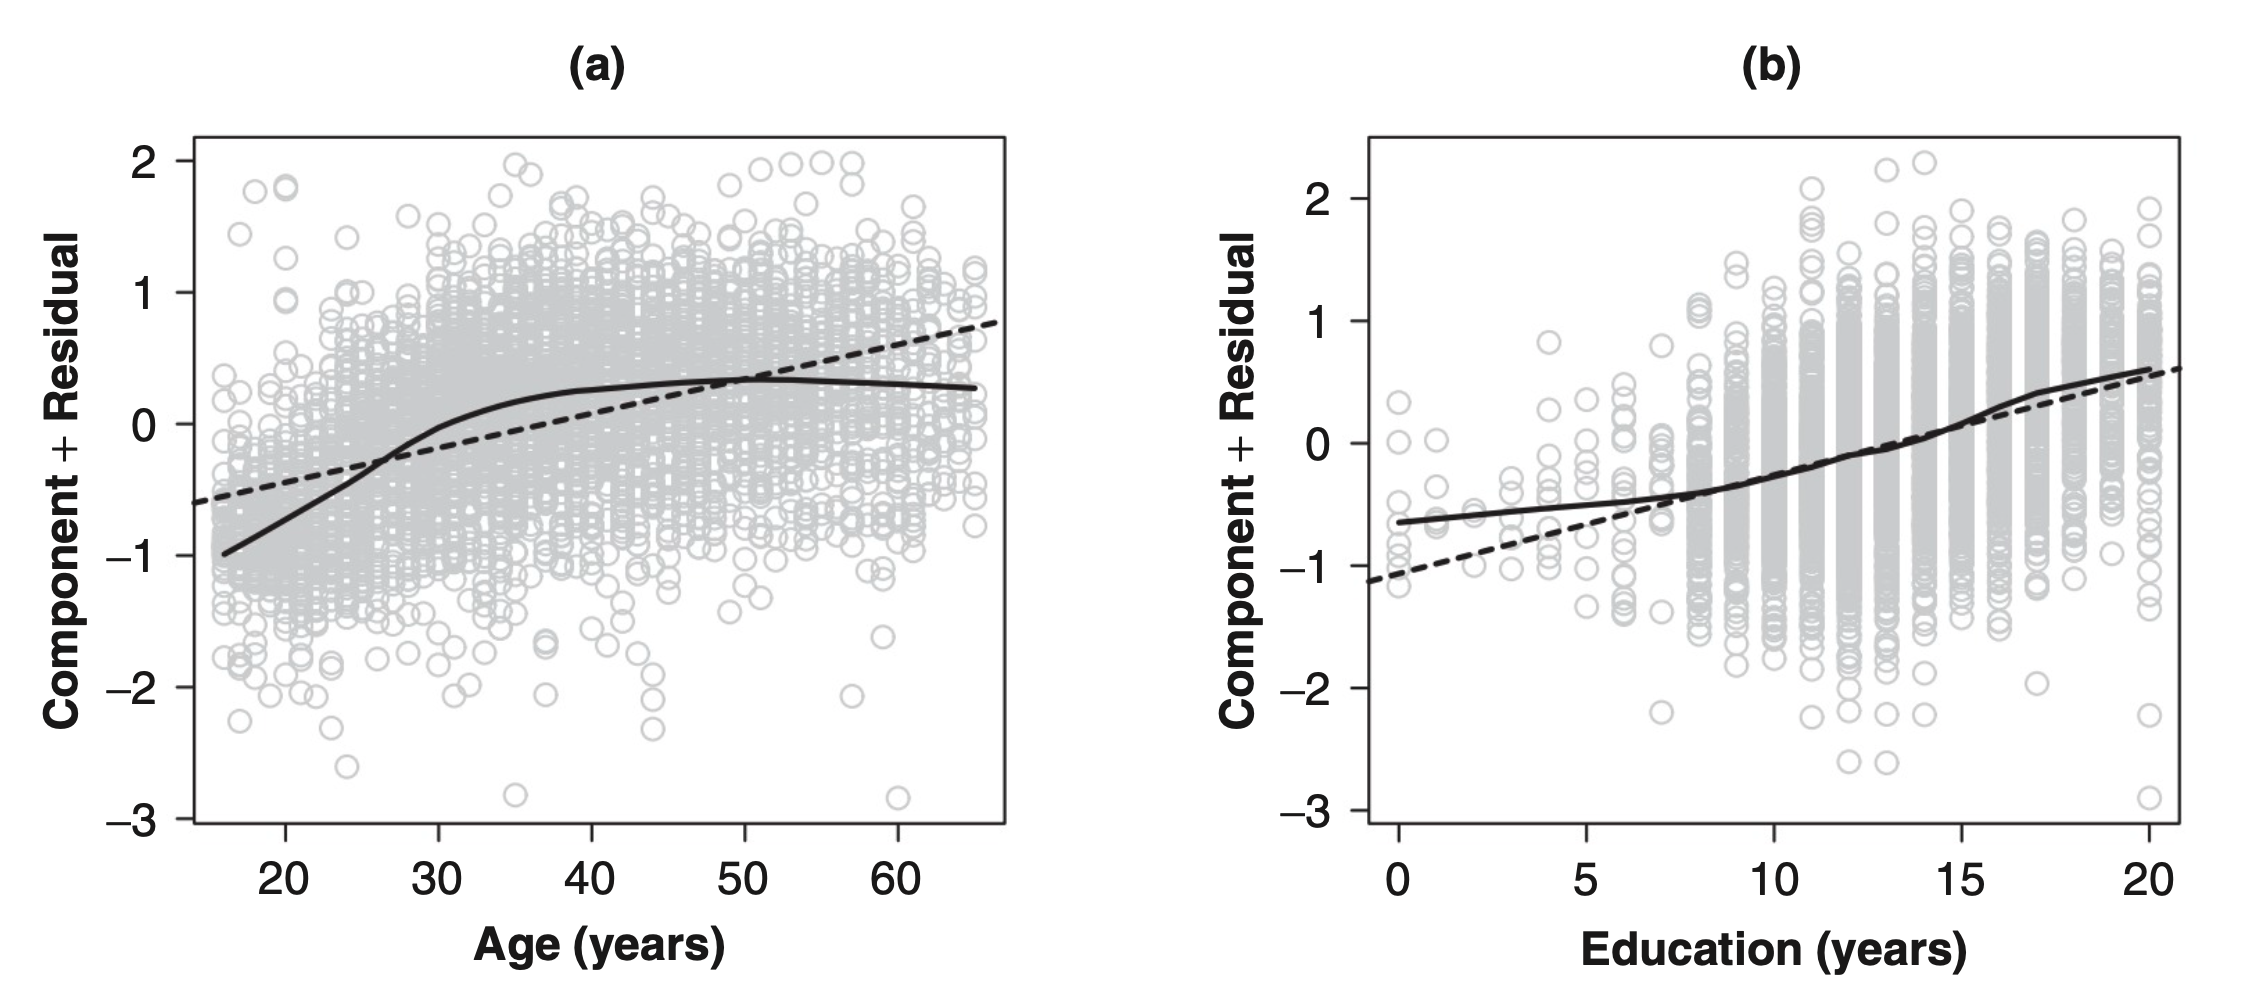
\includegraphics[width=0.9\textwidth]{Lecture19/JF_12_6}
  \caption{
  Component-plus-residual plots for age and education in SLID regression of log wages on these variables and sex.
  The solid lines are for lowess smooths with spans of $0.4$, and the broken lines are for linear least-squares fits.
   JF Figure 12.6.}
  \label{fig:JF_12_6}
\end{center}
\end{figure}
%



\subsection*{Data transformation}

%\subsubsection*{Transforming nonconstant spread, JF 4.4}
%An application of Tukey's rule for selecting a transformation is to use the linear ``trend'' of the spread-level plot to suggest a spread-stabilizing power transformation of the data.
%Express the linear fit as:
%$$
%\log \mbox{spread} \approx a + b \log \mbox{level}
%$$
%Then the corresponding spread-stabilizing transformation uses the power $p = 1 - b$ for the Box-Cox family of power transformation.

\subsubsection*{The family of powers and Roots, JF 4.1}
A particularly useful group of transformations is the ``family'' of powers and roots:
$$
X \to X^p
$$
wehre the arrow indicates that we intend to replace $X$ with the transformed variable $X^p$.
If $p$ is negative, then the transformation is an inverse power. For example, $X^{-1} = 1/X$.
If $p$ is a fraction, then the transformation represents a root.  For example, $X^{1/3} = \sqrt[3]{X}$.

It is more convenient to define the family of power transformations in a slightly more complex manner, called the \underline{Box-Cox family} of transformations (introduced in a seminal paper on transformations by Box \& Cox, 1964):
$$
X \to X^{(p)} = \frac{X^p - 1}{p}
$$

Because $X^{(p)}$ is a linear function of $X^p$, the two transformations have the same essential effect on the data, but, as is apparent in Figure~\ref{fig:JF_4_1}
%
\begin{figure}[H]
\begin{center}
  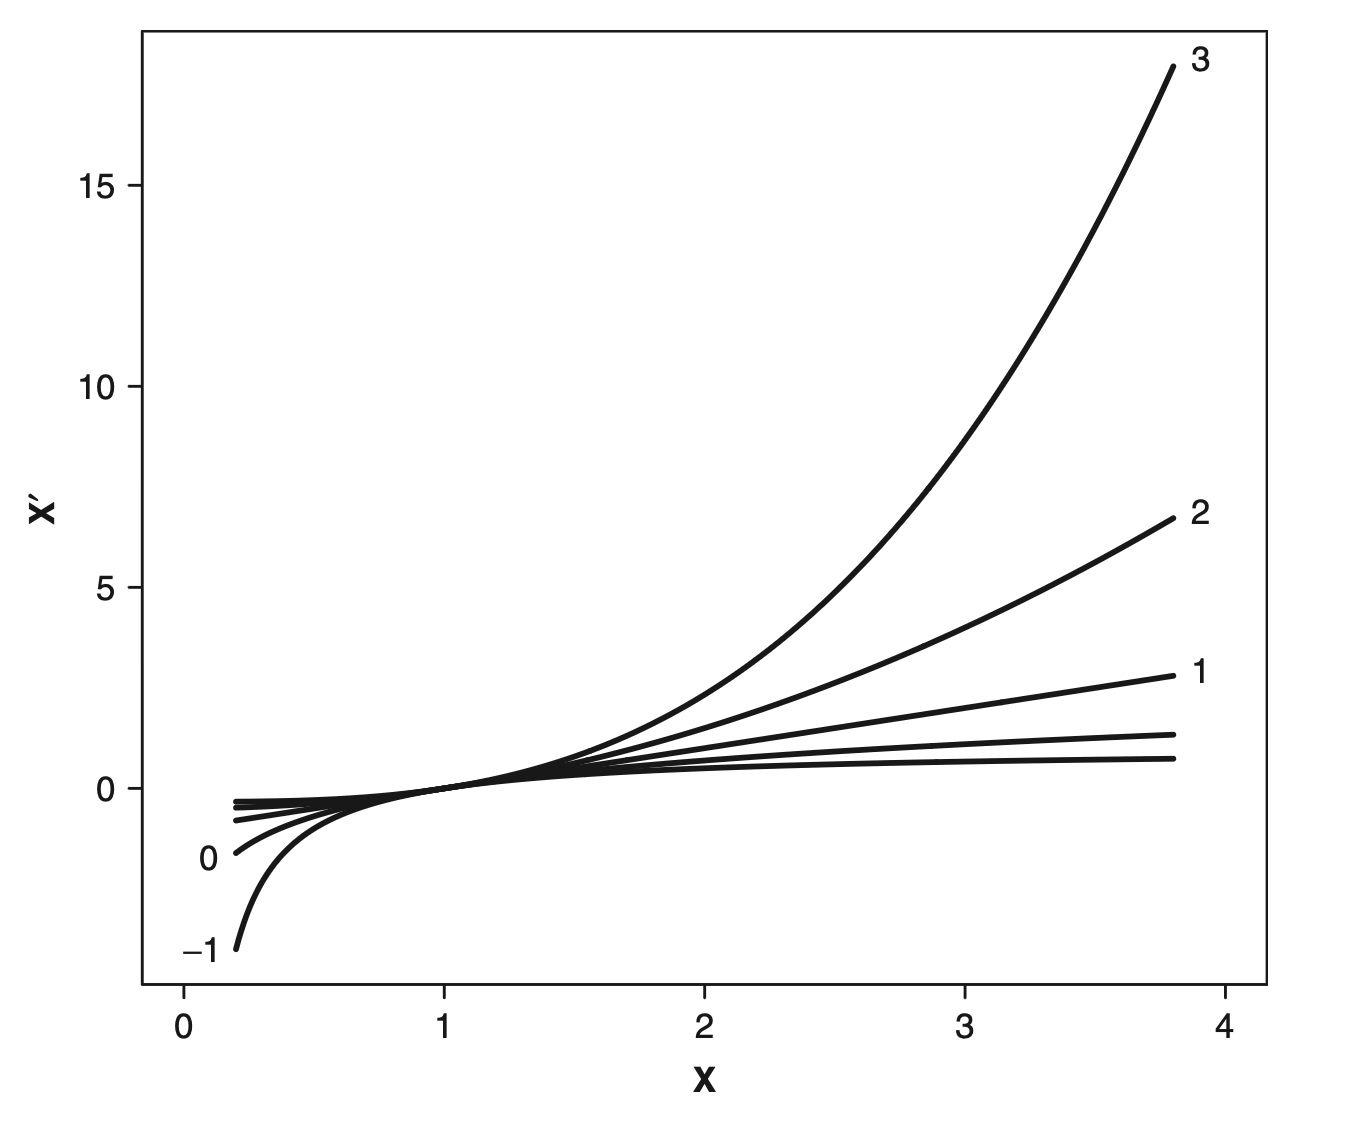
\includegraphics[width=0.8\textwidth]{Lecture18/JF_4_1}
  \caption{The Box-Cox family of power transformations $X'$ of $X$.
  The curve labeled $p$ is the transformation $X^{(p)}$, that is $(X^p - 1)/p$; $X^{(0)}$ is $\log_e(X)$.
   JF Figure 4.1.}
  \label{fig:JF_4_1}
\end{center}
\end{figure}
%
\begin{itemize}
  \item Dividing by $p$ preserves the direction of $X$, which otherwise would be reversed when $p$ is negative.
  \item The transformations $X^{(p)}$ are ``matched'' above $X=1$ both in level and in slope:
    \begin{enumerate}
      \item $1^{(p)} = 0$, for all values of $p$
      \item each transformation has a slope of $1$ at $X=1$.
    \end{enumerate}
  \item Descending the ``ladder'' of powers and roots towards $X^{(-1)}$ compresses the large values of $X$ and spreads out the small ones.
  Ascending the ladder of powers and roots towards $X^{(2)}$ has the opposite effect.
  As $p$ moves further from $p=1$ (i.e.~no transformation) in either direction, the transformation grows more powerful, increasingly ``bending'' the data.
  \item The power transformation $X^0$ is useless because it changes all values to $1$, but we can think of the log transformation as a kind of ``zeroth'' power:
  $$
  \lim\limits_{p \to 0} \frac{X^p - 1}{p} = \log_e X
  $$
  and by convention, $X^{(0)} \equiv \log_e X$.
\end{itemize}

\subsubsection*{Box-Cox transformation of $Y$}

Box and Cox (1964) suggested a power transformation of $Y$ with the object of normalizing the error distribution, stabilizing the error variance, and straightening the relationship of $Y$ to the $X$s.
The general Box-Cox model is
$$
Y_i^{(\lambda)} = \beta_0 + \beta_1 X_{i1} + \dots + \beta_p X_{ip} + \epsilon_i
$$
where $\epsilon_i \distas{iid} N(0, \sigma_\epsilon^2)$, and 
$$
Y_i^{(\lambda)} = \left\{ \begin{array}{ll}  
\frac{Y_i^\lambda - 1}{\lambda} & \mbox{for } \lambda \ne 0\\
\log_e Y_i & \mbox{for } \lambda = 0\\
 \end{array} \right.
$$
Note: in statistics, $\log_e$ is often written as $\log$.

For a particular choice of $\lambda$, the conditional maximized log-likelihood (see JF 12.5.1 p.324 footnote 55) is
$$
\begin{aligned}
\log_e L(\beta_0, \beta_1, \dots, \beta_p, \sigma_\epsilon^2 | \lambda) &= - \frac{n}{2} (1 + \log_e 2\pi)  \\
&-\frac{n}{2}\log_e \hat{\sigma}_\epsilon^2(\lambda) + (\lambda - 1)\sum\limits_{i = 1}^n \log_e Y_i\\
\end{aligned}
$$
where $\hat{\sigma}_\epsilon^2(\lambda) = \sum \hat{\epsilon}_i^2(\lambda) / n$ and where $\hat{\epsilon}_i(\lambda)$ are the residuals from the least-squares regression of $Y^{(\lambda)}$ on $X$s.
The least-squares coefficients from this regression are the maximum-likelihood estimates of $\beta$s conditional on the values of $\lambda$.

A simple procedure for finding the maximum-likelihood estimator $\hat{\lambda}$ is to evaluate the maximized $\log_e L$ (called the \underline{profile log-likelihood}) for a range of values of $\lambda$.
To test:$H_0: \lambda = 1$, calculated the likelihood-ratio statistic
$$
G_0^2 = -2 [\log_e L(\lambda = 1) - \log_e L(\lambda = \hat{\lambda})]
$$
which is asymptotically distributed as $\chi^2_1$ with one degree of freedom under $H_0$.
A 95\% confidence interval for $\lambda$ includes those values for which
$$
\log_e L(\lambda) > \log_e L(\lambda = \hat{\lambda}) - 1.92
$$
The number $1.92$ comes from $\frac{1}{2}\chi^2_{1, 0.05} = 0.5 \times 1.96^2$.

Figure~\ref{fig:JF_12_14} shows a plot of the profile log-likelihood against $\lambda$ for the original SLID regression of composite hourly wages on sex, age,  and education.
The maximum-likelihood estimate of $\lambda$ is $\hat{\lambda} = 0.09$, and a 95\% confidence interval runs from $0.04$ to $0.13$.
Although $0$ is outside of the CI (confidence interval), it is essentially the same transformation of wages as $\lambda=0.09$ (the correlation between log wages and wages${}^{0.09}$ is $0.9996$).
%
\begin{figure}[H]
\begin{center}
  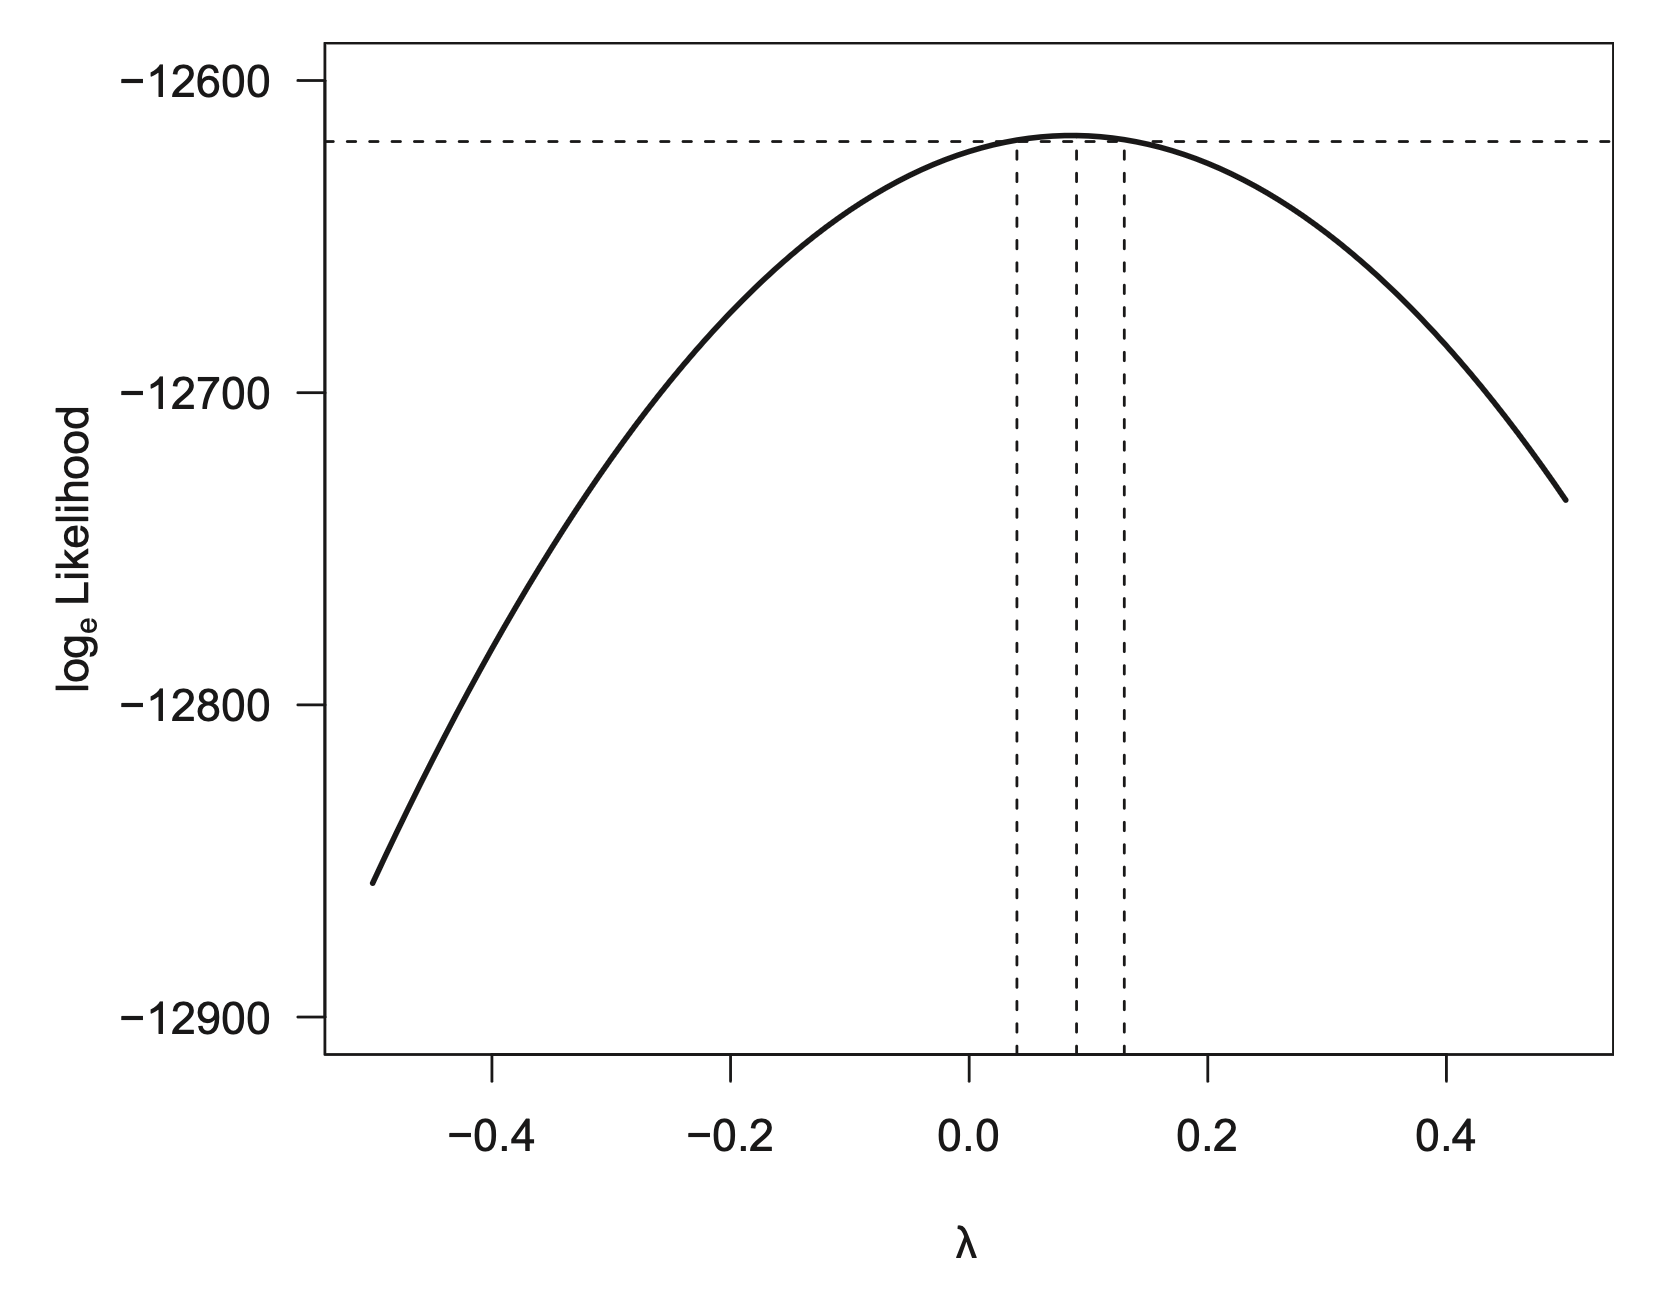
\includegraphics[width=0.6\textwidth]{Lecture19/JF_12_14}
  \caption{
  Box-Cox transformations for the SLID regression of wages on sex, age, and education.
  The maximized (profile) log-likelihood is plotted against the transformation parameter $\lambda$.
  The intersection of the line near the top of the graph with the profile log-likelihood curve marks off a 95\% confidence interval for $\lambda$.
  The maximum of the log-likelihood corresponds to the MLE of $\lambda$.
   JF Figure 12.14.}
  \label{fig:JF_12_14}
\end{center}
\end{figure}
%

\subsubsection*{Box-Tidwell transformation of $X$s}

Now, consider the model
$$
Y_i = \beta_0 + \beta_1 X_{i1}^{\gamma_1} + \dots +  \beta_p X_{ip}^{\gamma_p}  + \epsilon_i
$$
where the errors are independently distributed as $\epsilon_i \distas{iid} N(0, \sigma_\epsilon^2)$ and all the $X_{ij}$ are positive.

The parameters of this model ($\beta_0, \beta_1, \dots, \beta_p, \gamma_1, \dots, \gamma_p$, and $\sigma_\epsilon^2$) could be estimated by general nonlinear least squares.
Box and Tidwell (1962) suggested the following computationally more efficient procedure (also yields a constructed-variable diagnostic):
\begin{enumerate}
  \item Regress $Y$ on $X_1, \dots, X_p$, obtaining $\hat{\beta}_0, \hat{\beta}_1, \dots, \hat{\beta}_p$.  (``Regress $A$ on $B$s'' is the same as ``fitting the linear regression model with $A$ as the response variable and $B$s as the explanatory variables''.)
  \item Regress $Y$ on $X_1, \dots, X_p$ and the \underline{constructed variables} $X_1 \log_e X_1, \dots, X_p \log_e X_p$ (again, by fitting the model of $Y = \beta_0 + \beta_1 X_1 + \dots + \beta_p X_p + \delta_1 X_1 \log_e X_1 + \dots + \delta_p X_p \log_e X_p + \epsilon_i$) to obtain $\tilde{\beta}_0, \tilde{\beta}_1, \dots, \tilde{\beta}_p, \tilde{\delta}_1, \dots, \tilde{\delta}_p$.
  In general $\hat{\beta}_i \ne \tilde{\beta}_i$.  (The constructed variables result from the first-order Taylor-series approximation to $X_j^{\gamma_j}$ evaluated at $\gamma_j = 1$: $ X_j^{\gamma_j} \approx X_1 + (\gamma_1 - 1) X_1 \log_e X_1 $. )
  \item The constructed variable $X_j \log_e X_j$ can be used to assess the need for a transformation of $X_j$ by testing the null hypothesis $H_0:\delta_j = 0$.
  Added-variable plots for the constructed variables are useful for assessing leverage and influence on the decision to transform the $X$s.
  \item A preliminary estimate of the transformation parameter $\gamma_j$ (not the MLE) is
  $$
  \tilde{\gamma_j} = 1 + \frac{\tilde{\delta}_j}{\hat{\beta}_j}
  $$
  where $\tilde{\delta}_j$ is from step 2 and $\hat{\beta}_j$ is from step 1.
\end{enumerate}

\subsection*{Polynomial regression}
A machinery of multiple regression to fit non-linear relationships between predictor(s) and response.
\begin{itemize}
  \item Linear: $y = \beta_0 + \beta_1 x + \epsilon$
  \item Quadratic: $y = \beta_0 + \beta_1 x + \beta_2 x^2 + \epsilon$
  \item Cubic: $y = \beta_0 + \beta_1 x  +\beta_2 x^2 + \beta_3 x^3 + \epsilon$ 
  \item $k^{th}$ order polynomial:  $y = \beta_0 + \beta_1 x + \beta_2 x^2 + \dots +\beta_k x^k + \epsilon$
\end{itemize}

Question:\\
Does quadratic model provide a significantly better fit than linear model?\\
{\it Solution: }Test $H_0: \beta_2 = 0$ vs. $H_a: \beta_2 \ne 0$.\\
Alternatively, compare the corresponding adjusted-$R^2$ values.















